%% -*- coding: utf-8 -*-
\documentclass[12pt,pagesize,paper=landscape,paper=192mm:108mm]{scrbook} 
%1920x1080 1280x720
\areaset[current]{192mm}{108mm}
\usepackage{calc}
\usepackage[T2A]{fontenc}
\usepackage[utf8]{inputenc}
\usepackage[english,russian]{babel}
\usepackage{microtype}
\usepackage{misccorr}
\usepackage{cmap}
%\usepackage[unicode=true]{hyperref}
\usepackage{graphicx}
\usepackage{amssymb}
\usepackage{amsmath}
%\usepackage{srcltx}
\usepackage{textcomp}
\usepackage{xspace}
%научные символы и смайлики \smiley \frownie
\usepackage{wasysym}
\usepackage{ccicons}
\begin{document}
\begin{titlepage}
  \vspace*{-0.5em}
  \begin{center}    
    \hspace*{3em}
    \begin{minipage}[t]{3em}
      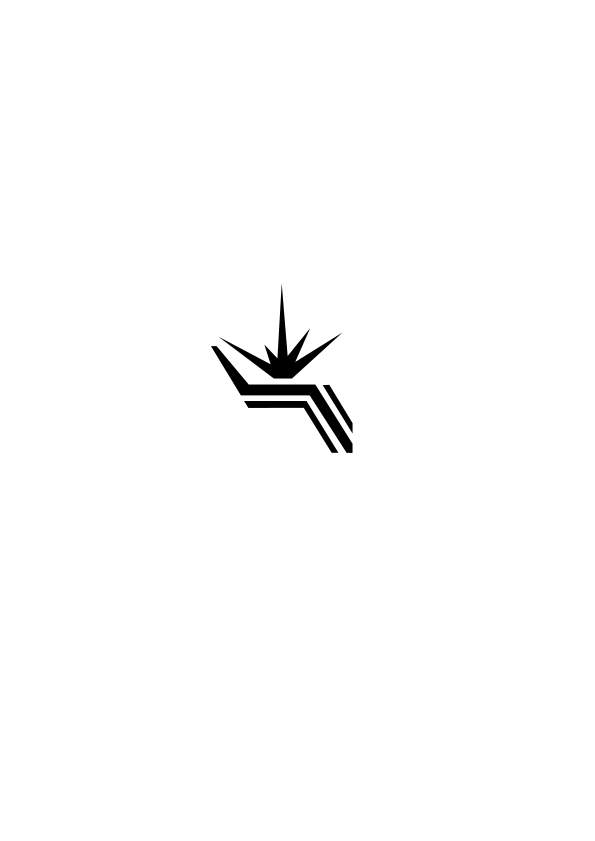
\includegraphics[width=\textwidth]{../BINP-logo}
    \end{minipage}\hfill
    \begin{minipage}{0.23\linewidth}
    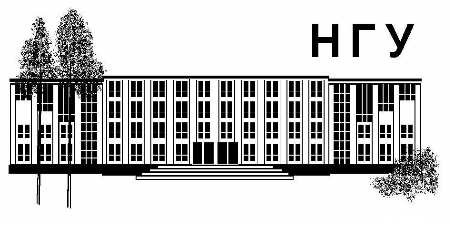
\includegraphics[width=\textwidth]{../NSU-logo}
    \end{minipage}
    \hfill
    \hspace*{6em}

    Кафедра теоретической физики физического факультета НГУ
    \medskip

    \Large
    Профессор Фадин В.\,С.
    \bigskip

    \huge
    \textbf{Квантовая электродинамика}
    \bigskip

    \Large
    Лекция № 3
    \vfill

    \normalsize
    % \begin{minipage}{0.65\linewidth}
    % \end{minipage}
    \vfill

    \normalsize \ccbysa\hspace{0.5em}  Новосибирск 2013
  \end{center}
\end{titlepage}
\newpage

\vspace*{-1em}
\begin{center}
\vfill
  \begin{minipage}{0.65\linewidth}
    Вероятность распада частицы. Фазовый объем конечных
    состояний. Сечение рассеяния.  Процессы рассеяния во внешнем поле:
    лагранжиан взаимодействия, правила Фейнмана, плотность конечных
    состояний, сечение рассеяния. Поляризация начальных и конечных
    состояний. Спиновая волновая функция
    электрона. Эрмитовосопряженный матричный элемент, сведение
    вычисления квадрата матричного элемента к вычислению
    следов. Полный набор в пространстве эрмитовых матриц $4 \times
    4$. Поляризационные матрицы плотности для электрона и
    позитрона. Поляризация частиц в конечном
    состоянии. Поляризационное состояние фотонов, матрица плотности,
    параметры Стокса. Суммирование по поляризациям фотона,
    ковариантное (фейнмановское) суммирование с учетом калибровочной
    инвариантности (сохранения тока), сокращение вкладов временных и
    продольных фотонов.  Кросс"=инвариантность, различные каналы
    реакции, поведение поляризации при кроссинге.
  \end{minipage}
  \vfill

  % \normalsize \ccbysa\hspace{0.5em} Новосибирск 2013
\end{center}
\end{document}
